\documentclass[12pt,a4paper]{article}

\usepackage[utf8]{inputenc}
\usepackage[T1]{fontenc}
\usepackage{polski}

\usepackage{amsthm}
\usepackage{amsmath}
\usepackage{amsfonts}
\usepackage{amssymb}
\usepackage{pgfplots}
\usepackage{tikz}
\usepackage{lmodern}	%fancy font
\usepackage{textcomp}

\usepackage{indentfirst}
\usepackage{graphicx}
\usepackage{caption}
\usepackage{subcaption}
\usepackage{siunitx}
\usepackage{here}


\setlength{\textheight}{24cm}
\setlength{\textwidth}{15.92cm}
\setlength{\footskip}{10mm}
\setlength{\oddsidemargin}{0mm}
\setlength{\evensidemargin}{0mm}
\setlength{\topmargin}{0mm}
\setlength{\headsep}{5mm}
\usepackage{tikz}
\usepackage{lmodern}	%fancy font
\usepackage{textcomp}

\usepackage{indentfirst}
\usepackage{graphicx}
\usepackage{caption}
\usepackage{subcaption}
\usepackage{siunitx}
\usepackage{here}
\usepackage[margin=1in]{geometry}% Just for this example
\setlength{\parindent}{0pt}% Just for this example
\setlength{\textheight}{24cm}
\setlength{\textwidth}{15.92cm}
\setlength{\footskip}{10mm}
\setlength{\oddsidemargin}{0mm}
\setlength{\evensidemargin}{0mm}
\setlength{\topmargin}{0mm}


\begin{document}

\begin{table}[H]
\label{my-label}
\begin{tabular}[width=\textwidth, height=0.5]{|c|c|}
\hline
									           					&                           \\

\includegraphics[height=3cm]{logo}             					& \textbf{Technika cyfrowa} \\ \hline
\multicolumn{1}{|l|}{\textbf{Temat ćwiczenia}} 					& \textbf{Numer ćwiczenia}  \\
\multicolumn{1}{|l|}{Minimalizacja i praktyczna realizacja złożonych funkcji logicznych}	& 2                         \\ \hline
\multicolumn{1}{|l|}{\textbf{Wykonawca}}       & \textbf{Ocena}            \\
\multicolumn{1}{|l|}{Łukasz Nawojowski}          &                           \\ \hline
\end{tabular}
\end{table}

\section{Cel ćwiczenia}
Zapoznanie się z zastosowaniem tablic Karnaugh'a do minimalizacji graficznej złożonych funkcji logicznych oraz zaprojektowanie w Multisimie układu cyfrowego zwiększającego o 1 trzybitową liczbę całkowitą oraz wyświetlacza siedmiosegmentowego.

\section{Przebieg ćwiczenia}
\subsection{Inkrementator trzybitowych liczb całkowitych}
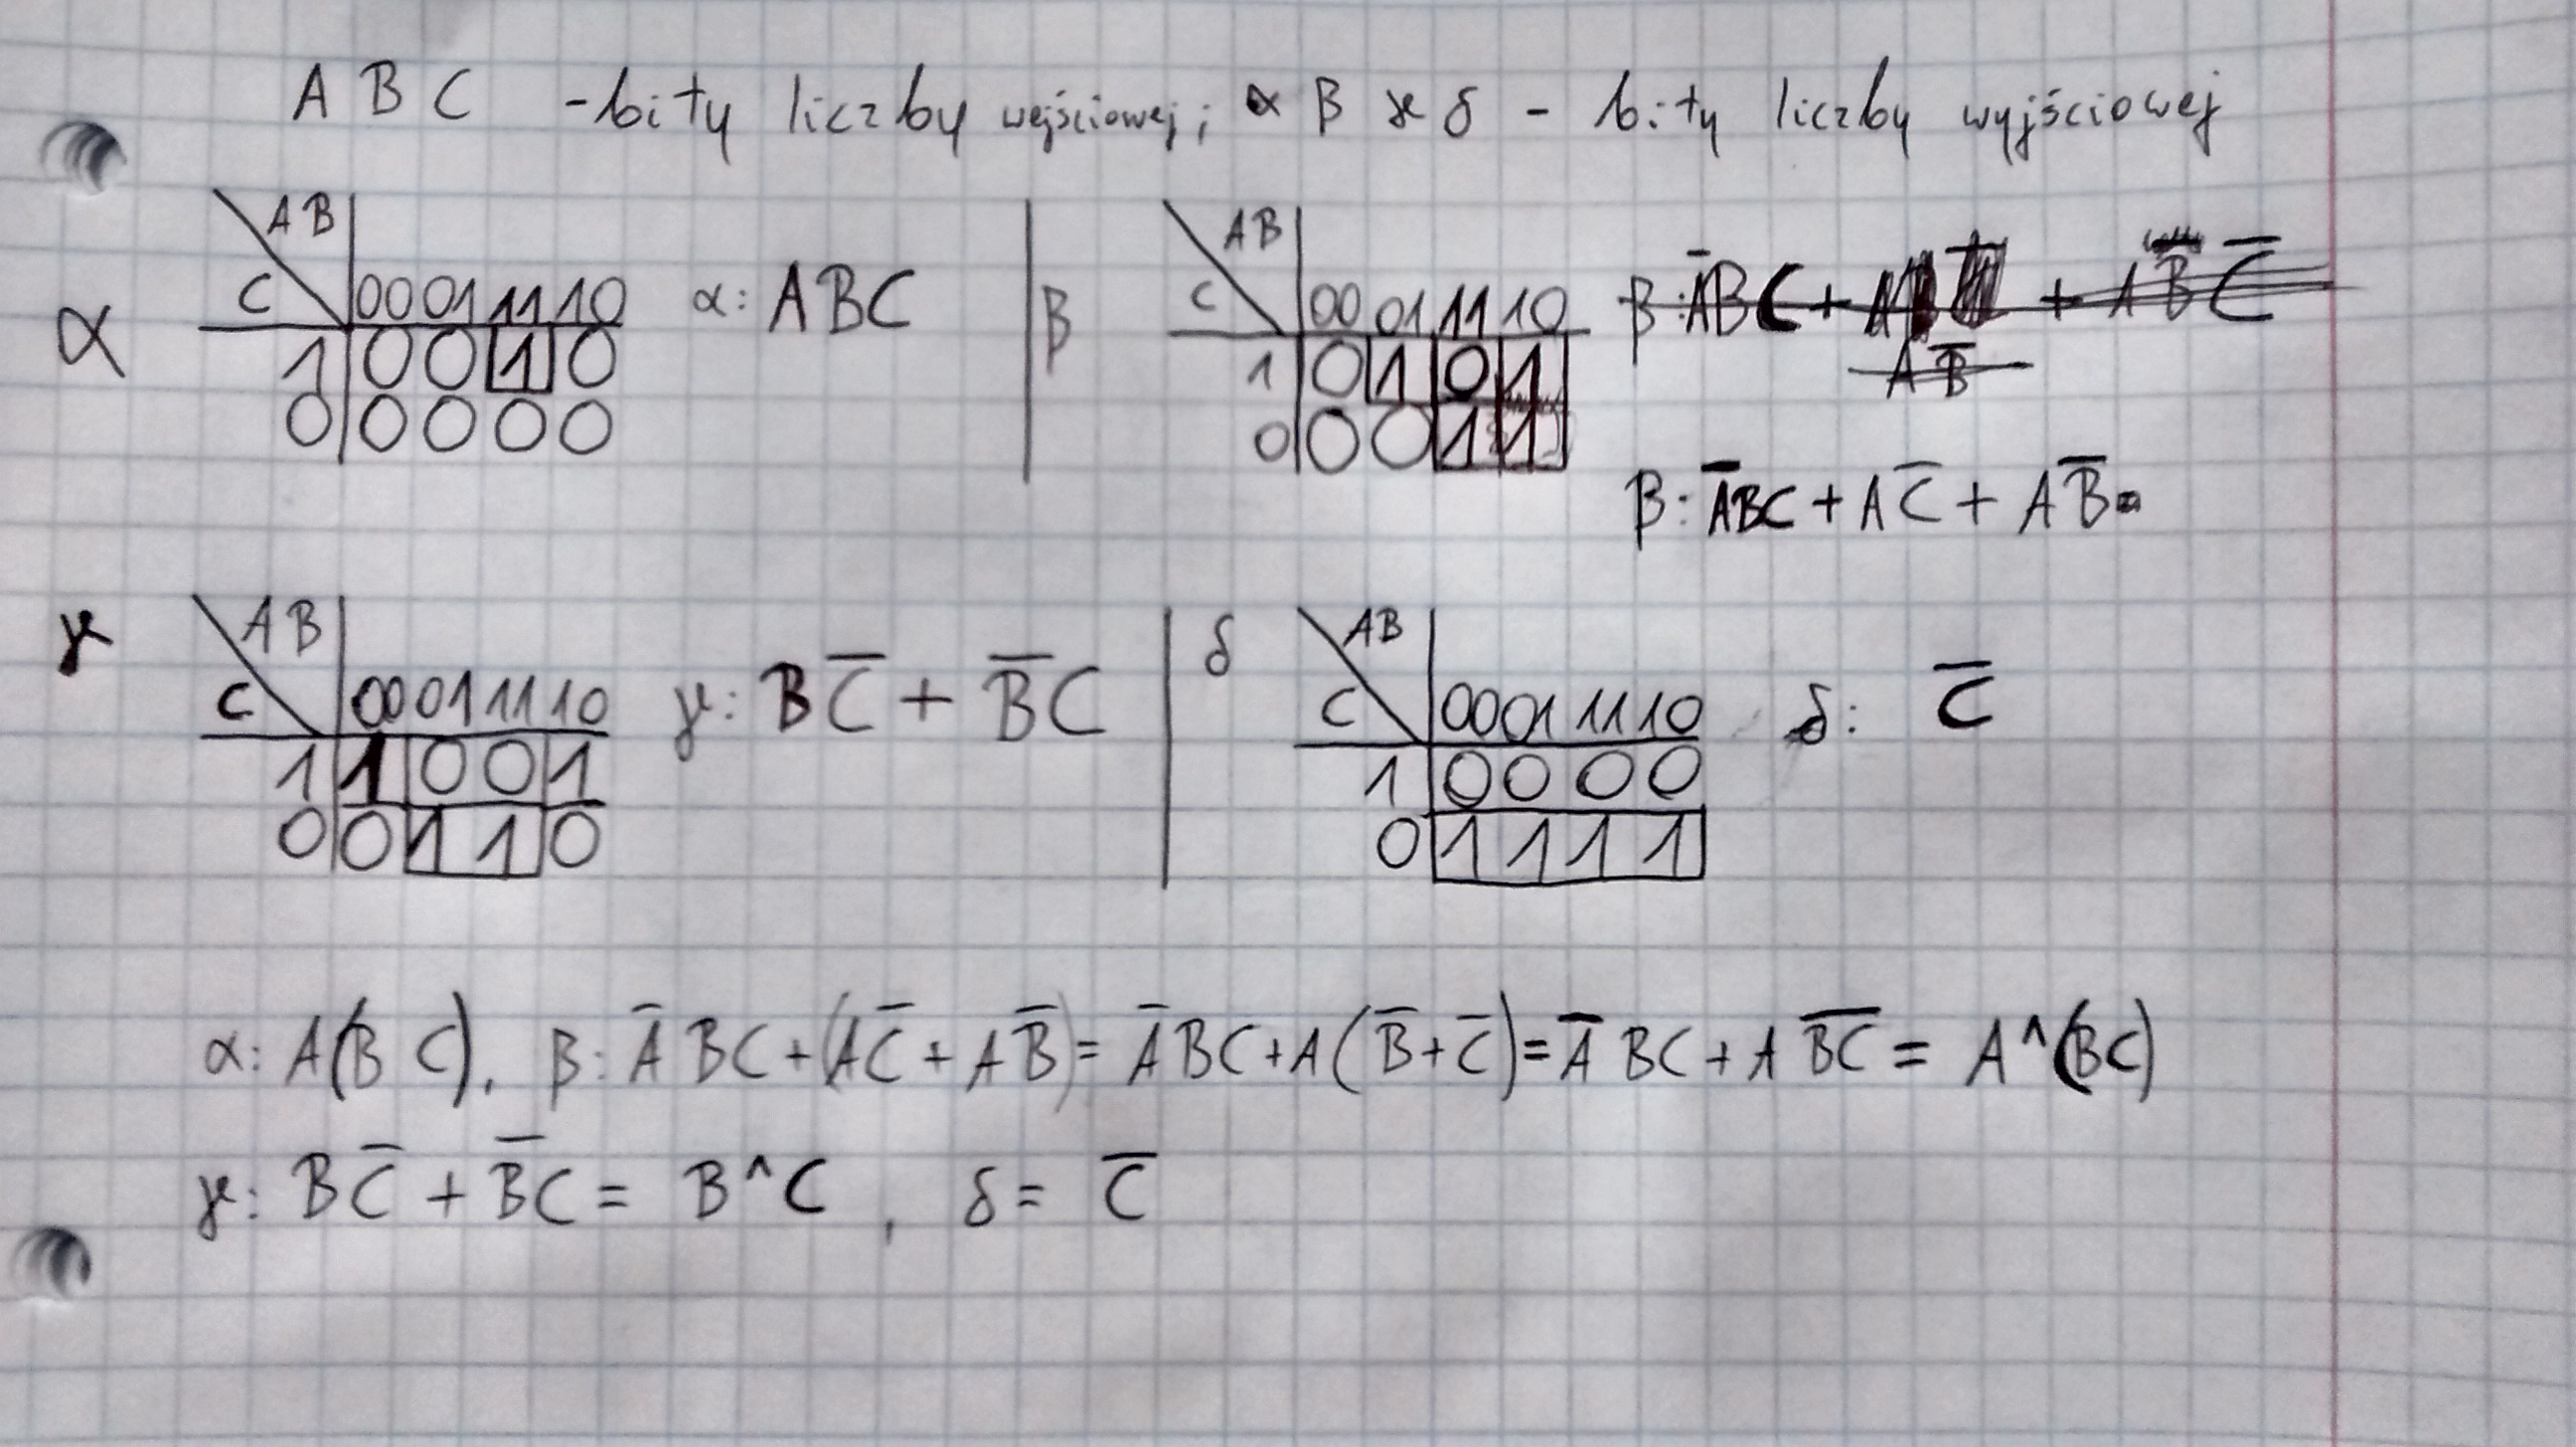
\includegraphics[width=\textwidth]{7_bit_incr_karnaugh}
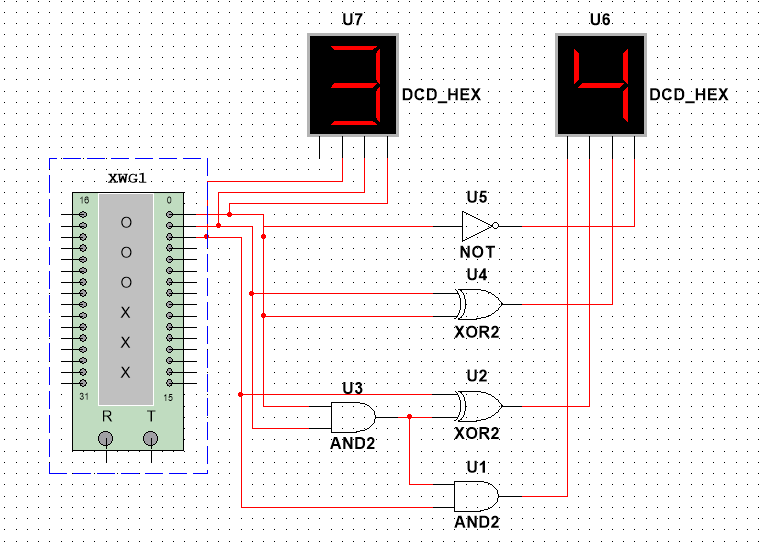
\includegraphics[width=\textwidth]{2aBetter}


\subsection{Minimalizacja funkcji metodą tablic Karnaugha}
Zadaną funkcję logiczną zminimalizowano za pomocą tablicy Karnaugh:

\begin{figure}[H]
\centering
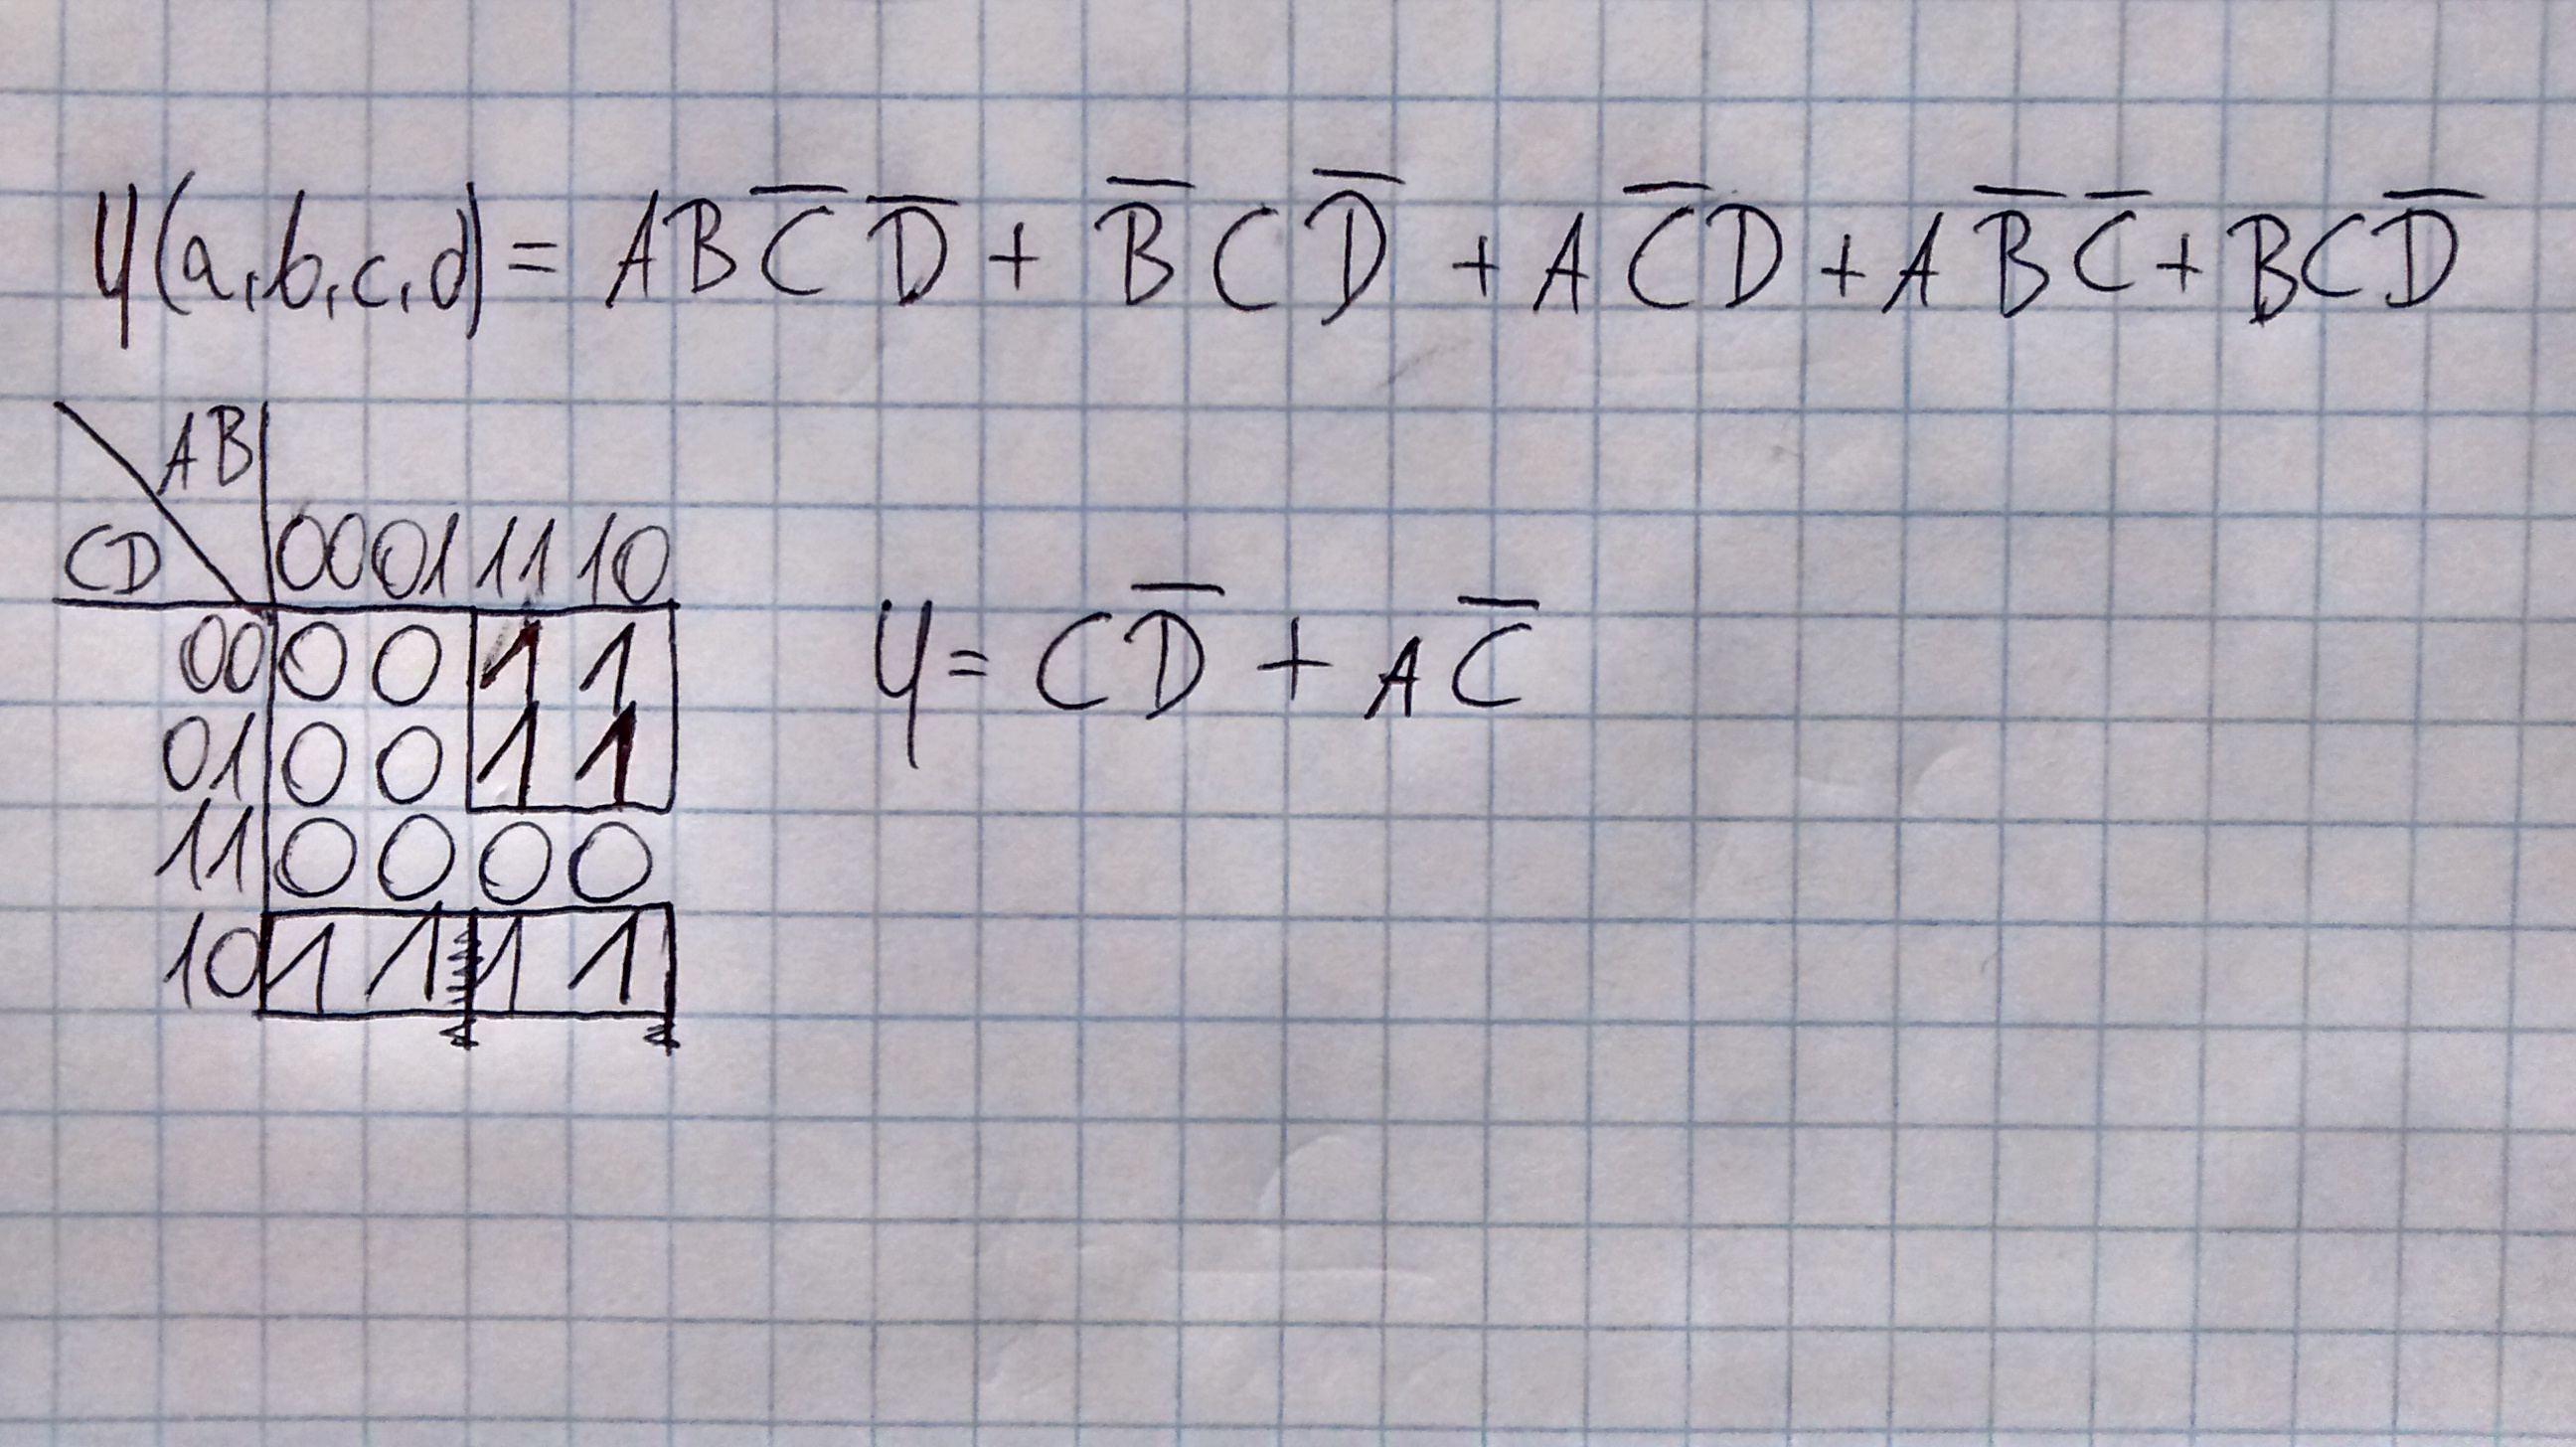
\includegraphics[width=\textwidth]{min_func_karnaugh}
\end{figure}

Porównano zminimalizowaną funkcję z funkcją wejściową:

\begin{figure}[H]
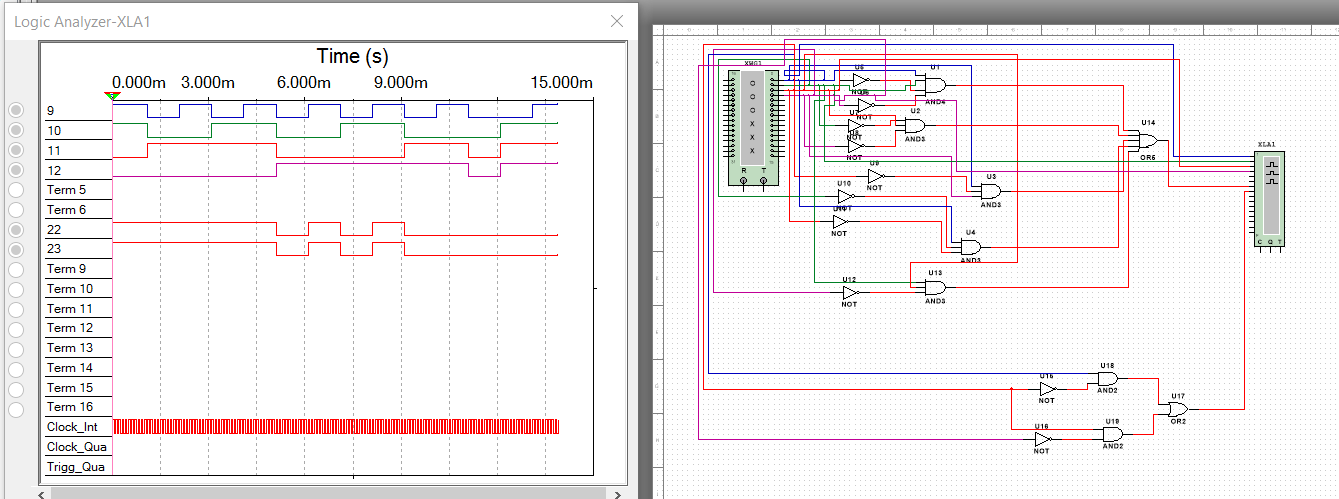
\includegraphics[width=\textwidth]{2b}
\end{figure}

\newpage
\subsection{Transkoder czterobitowych cyfr}
W oparciu o poniższą konfigurację segmentów:

\begin{figure}[H]
\centering
\includegraphics[width=0.25\textwidth]{7seg/segconf}
\end{figure}

Dla każdego z siedmiu segmentów zrealizowano tablicę Karnaugha prezentującą pożądane zachowanie segmentu, zminimalizowano funkcję logiczną i zbudowano odpowiedni obwód.

\subsubsection{Segment a}
\begin{figure}[H]
\centering
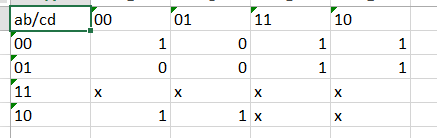
\includegraphics[width=0.3\textwidth]{7seg/seg0}
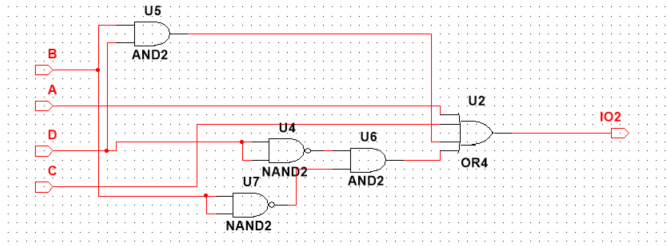
\includegraphics[width=\textwidth]{7seg/seg0circ}
\end{figure}

\newpage
\subsubsection{Segment b}
\begin{figure}[H]
\centering
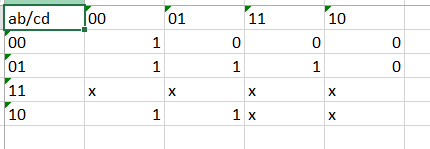
\includegraphics[width=0.3\textwidth]{7seg/seg1}
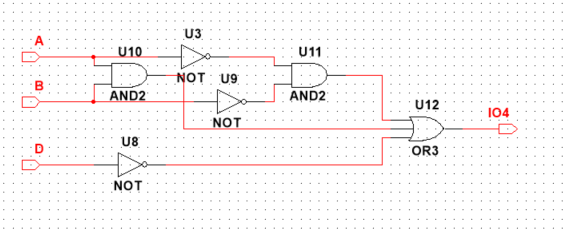
\includegraphics[width=0.7\textwidth]{7seg/seg1circ}
\end{figure}

\subsubsection{Segment c}
\begin{figure}[H]
\centering
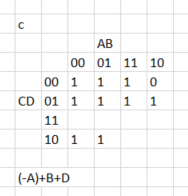
\includegraphics[width=0.3\textwidth]{7seg/seg2}
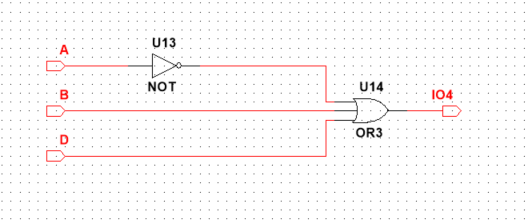
\includegraphics[width=0.7\textwidth]{7seg/seg2circ}
\end{figure}

\newpage
\subsubsection{Segment d}
\begin{figure}[H]
\centering
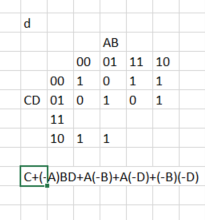
\includegraphics[width=0.3\textwidth]{7seg/seg3}
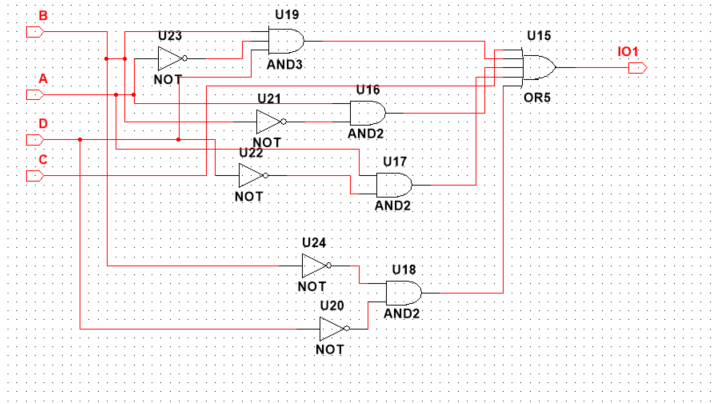
\includegraphics[width=0.7\textwidth]{7seg/seg3circ}
\end{figure}

\subsubsection{Segment e}
\begin{figure}[H]
\centering
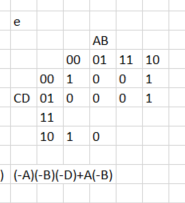
\includegraphics[width=0.3\textwidth]{7seg/seg4}
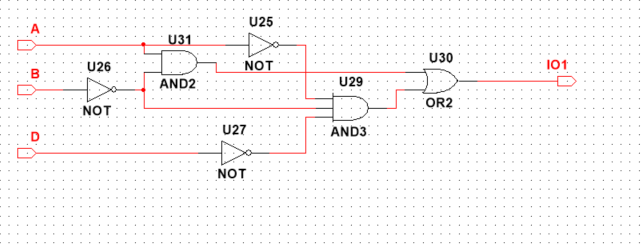
\includegraphics[width=0.7\textwidth]{7seg/seg4circ}
\end{figure}

\newpage
\subsubsection{Segment f}
\begin{figure}[H]
\centering
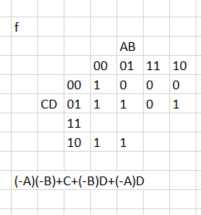
\includegraphics[width=0.3\textwidth]{7seg/seg5}
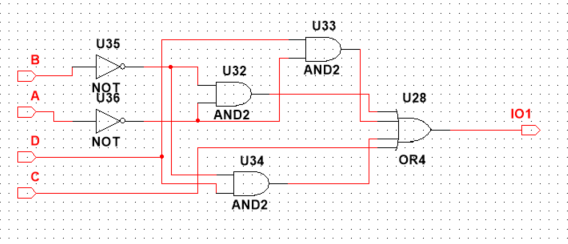
\includegraphics[width=0.7\textwidth]{7seg/seg5circ}
\end{figure}

\subsubsection{Segment g}
\begin{figure}[H]
\centering
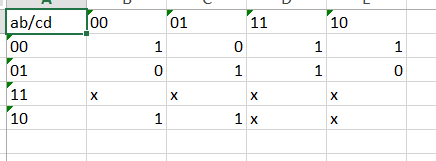
\includegraphics[width=0.3\textwidth]{7seg/seg6}
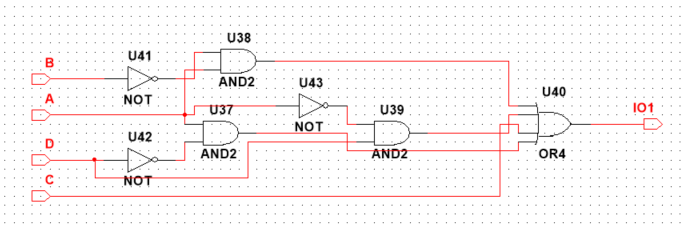
\includegraphics[width=0.7\textwidth]{7seg/seg6circ}
\end{figure}

\newpage
Obwody podłączono do wyświetlacza siedmiosegmentowego i przetestowano. Wyświetlacz wskazywał przewidywane cyfry:

\begin{figure}[H]
\centering
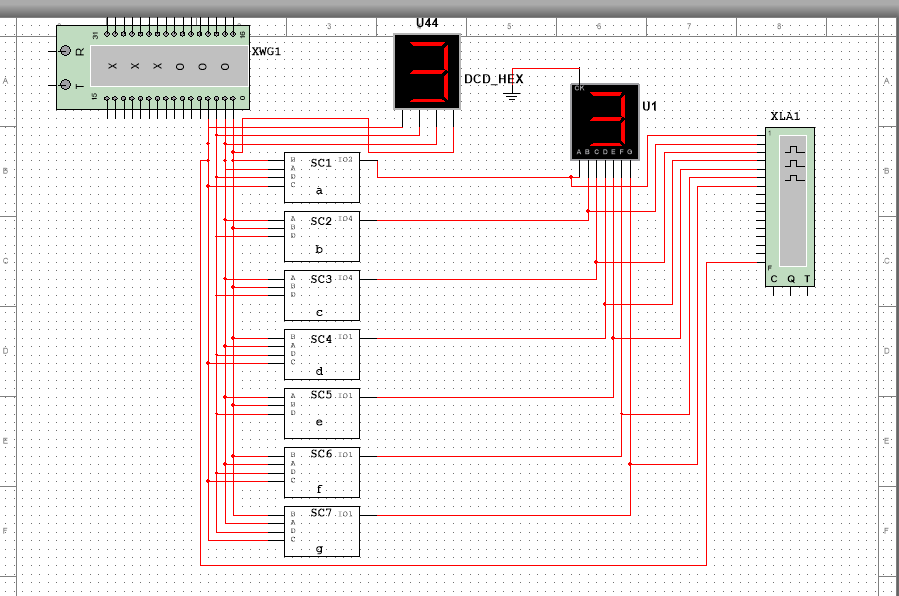
\includegraphics[width=\textwidth]{7seg/7segall}
\end{figure}

\end{document}
